\documentclass[12pt,a4paper,oneside]{article}
\usepackage[utf8]{inputenc}
\usepackage{t1enc} % hyphenate accented chars
\usepackage[hungarian]{babel}
\usepackage{../fedlap}
\usepackage{fancyhdr} % elofej, elolab
\usepackage{graphicx}
\usepackage{datetime} % specify date format
\setcounter{secnumdepth}{3} % enable subsubsection

% hasonlitson a doc verziora
\addtolength{\voffset}{-1cm}

% cim
\csapat{nand}{39}
\konzulens{Bozóki Szilárd}
\datum{\todaynum}

% csapattagok
\taga{Berki Endre}{HQNHER}{berkiendre@gmail.com}
\tagb{Fodor Bertalan Ferenc}{H4T1UX}{foberci@gmail.com}
\tagc{Kádár András}{JFENWR}{arycika@gmail.com}
\tagd{Thaler Benedek}{EDDO10}{thalerbenedek@gmail.com}

\setlength{\headheight}{1.3em}
\setlength{\headsep}{2em}

% elofej, elolab
\fancyhf{}

\fancyhead[OL] { \tiny \leftmark{} }
\fancyhead[OR] { \tmpcsapat }

\fancyfoot[OR] { \thepage }
\fancyfoot[OL] { \tmpdatum }

\pagestyle{fancy}

% custom date format, according to customer request
% you have to use the \todaynum command instead of today,
% becouse babel overrides it, and I couldn't find a way to override
% it again. I was tempted to call this format \todaybozoki
\newcommand{\todaynum}{\the\year. \twodigit\month. \twodigit\day}


\usepackage{enumitem}
\usepackage{textcomp}
\usepackage[utf8]{inputenc}
\usepackage[T1]{fontenc}

\begin{document}

\anyag{7. Prototípus koncepciója}
\fedlap

\addtocounter{section}{6}
\section{Prototípus koncepciója}

	\subsection{Prototípus interface-definíciója}
	%Definiálni kell a teszteket leíró nyelvet. Külön figyelmet kell fordítani arra, hogy ha a rendszer véletlen elemeket is tartalmaz, akkor a véletlenszerűség ki-bekapcsolható legyen, és a program determinisztikusan is tesztelhető legyen.
	    \subsubsection{Az interfész általános leírása}
	    %A protó (karakteres) input és output felületeit úgy kell kialakítani, hogy az input fájlból is vehető legyen illetőleg az output fájlba menthető legyen, vagyis kommunikációra csak a szabványos be- és kimenet használható.
	    A prototípus célja, hogy képet kapjunk a szkeletonban külön-külön tesztelt kommunikációs egységek integrálás utáni helyes működéséről. A prototípus egyrészről tehát egy integrációs teszt, másrészről viszont egyszerre egy működőképes program is, mely az egyszerűség érdekében nélkülözi a grafikus felületet, parancssoros kommunikációt használ. A felhasználó a tesztelés során a prototípussal parancsok útján léphet interakcióba, így befolyásolva annak futását. A parancsok futtatása után a kimenet összevethető a specifikációval.
	    
	    \subsubsection{Bemeneti nyelv}
	    %Definiálni kell a teszteket leíró nyelvet. Külön figyelmet kell fordítani arra, hogy ha a rendszer véletlen elemeket is tartalmaz, akkor a véletlenszerűség ki-bekapcsolható legyen, és a program determinisztikusan is futtatható legyen. A szálkezelést is tesztelhető, irányítható módon kell megoldani.
	    %Parancs1 \ Leírás: \ Opciók:
	    
	    A felhasználó a következő parancsok állnak rendelkezésére a tesztelés során:
	    
	    \newcommand{\cmd}[1]{\item{\texttt{#1}} }
	    \begin{description}
	        \cmd{timerStart}: Óraütések automatikus kiadásának bekapcsolása.
	        \cmd{timerStop}: Óraütések automatikus kiadásának kikapcsolása.
	        \cmd{tick} \emph{count}: Megadott számú öraütést szimulál.
	        \cmd{loadMap} \emph{mapId}: Megadott pálya betöltése.
	        \cmd{move} \emph{stickmanId} \emph{direction}: A megadott azonosítójú stickman megfelelő irányba mozgatása (up, right, down, left).
	        \cmd{viewportSwitch}: Pálya és közeli nézet közötti váltás.
	        \cmd{moveFrame} \emph{direction}: Keret mozgatása pályanézetben a megadott irányba (up, right, down, left).
	        \cmd{echoCommands} \emph{status}: Bemeneti parancsok kiírása a kimenetre a könnyebb debuggolás kedvéért. (status: true vagy false)
        \end{description}
        
        A parancsokat a program a szabványos bemenetről olvassa be, így tetszőleges fájl beállítható a parancsok forrásának, ha a megfelelő fájlt a bemenetre irányítjuk.
        
        \subsubsection{Pálya fájlreprezentációja}
        %Ha szükséges, meg kell adni a konfigurációs (pl. pályaképet megadó) fájlok nyelvtanát is.
        A felhasznált pályákat a program fájlokból olvassa be, melyek felépítése a következő: A fájlok soralapúak, minden sor egy objektumot kódol a pályán. A sor elején a konkért objektumot azonosító név áll, majd egy tabulátorral elválasztva következnek a paraméterei. A különböző objektumok tetszőleges számú paramétert vehetnek át, mely paramétereket tabulátorral elválasztva kell az objektum neve után felsorolni. Minden, a pályán szereplő objektum első 4 paramétere (ha specifikált), rendre a következő attribútumokat kódolja: Pálya bal felső sarkától számított (abszolút) x irányú eltolás, y irányú eltolás, objektum szélessége, objektum magassága. A pálya fájlban a következő objektumnevek szerepelhetnek: \texttt{Door, Key, Platform, Stickman}. A pályán található keretek számának és elhelyezkedésének megadására nincs szükség, azt a program az elhelyezett elemek pozíciója alapján dinamikusan építi fel.
        
	    \subsubsection{Kimeneti nyelv}	
	    %Egyértelműen definiálni kell, hogy az egyes bemeneti parancsok végrehajtása után előálló állapot milyen formában jelenik meg a szabványos kimeneten.	
	    A karakteres kimeneten minden -- a modell állapotának változását okozó -- esemény, valamint bármely parancs után megjelenik a modell aktuális állapotát reprezentáló szöveges ábra. Alapértelmezetten nem, de az \texttt{echoCommands} parancs használatával a megadott parancs is kiírásra kerül pályarajz után, így segítve a kimenet követését, ha azt fájlba írtuk. A pálya szöveges reprezentációját képező ábrán a következő szimbólumok fordulhatnak elő:
	    
	    \begin{description}
	        \newcommand{\frameitem}[1]{\item{\textbf{#1}} }
	        % pdflatex doesn't accept the following symbols, use simpler ones
	        % ☺, ☻, █, ⚷, ☐
	        \frameitem{X, Y}: A stickmanek
	        \frameitem{|, --, +}: Keret függőleges széle, keret vízszintes széle, keret sarka
	        \frameitem{\#}: Platform
	        \frameitem{K}: Kulcs
	        \frameitem{A}: Ajtó
        \end{description}

        A pálya szöveges reprezentációja például az alábbi formát öltheti:
        
		\begin{figure}[hb]
		  \begin{center}
		  % let me introduce the centering of dummy people
		\begin{verbatim}
                +----------+ +----------+ +----------+
                |          | |        ##| |#        #|
                |  X##   ##| |##        | |#   K     |
                |##########| |##########| |##########|
                +----------+ +----------+ +----------+
                +----------+ +----------+
                |##   K    | |##     ###|
                |    ##    | |    Y   A |
                |##########| |##########|
                +----------+ +----------+
		\end{verbatim}
		  \caption{A pálya szöveges reprezentációja}
		  \end{center}
		\end{figure}        
        
        Mivel a program a kimenetét sztandard kimenetre írja ki, így az egyszerűen elemezhető a konzolon vagy írható fájlba. Amennyiben egy stickman megérint egy kulcsot, a kulcs eltűnik és a megszerzője tulajdonába kerül.
	
	\subsection{Összes részletes use-case}
        %domain specific commands
        \newcommand{\ucitem}[1]{\item \textbf{Név: #1}\\}
        \newcommand{\ucdesc}[1]{\textbf{Rövid leírás: } #1\\}
        \newcommand{\ucact}[1]{\textbf{Actor: } #1\\}
        \newcommand{\ucscenario}[1]{\textbf{Forgatókönyv: }#1\\}
        
		\begin{center}	
		    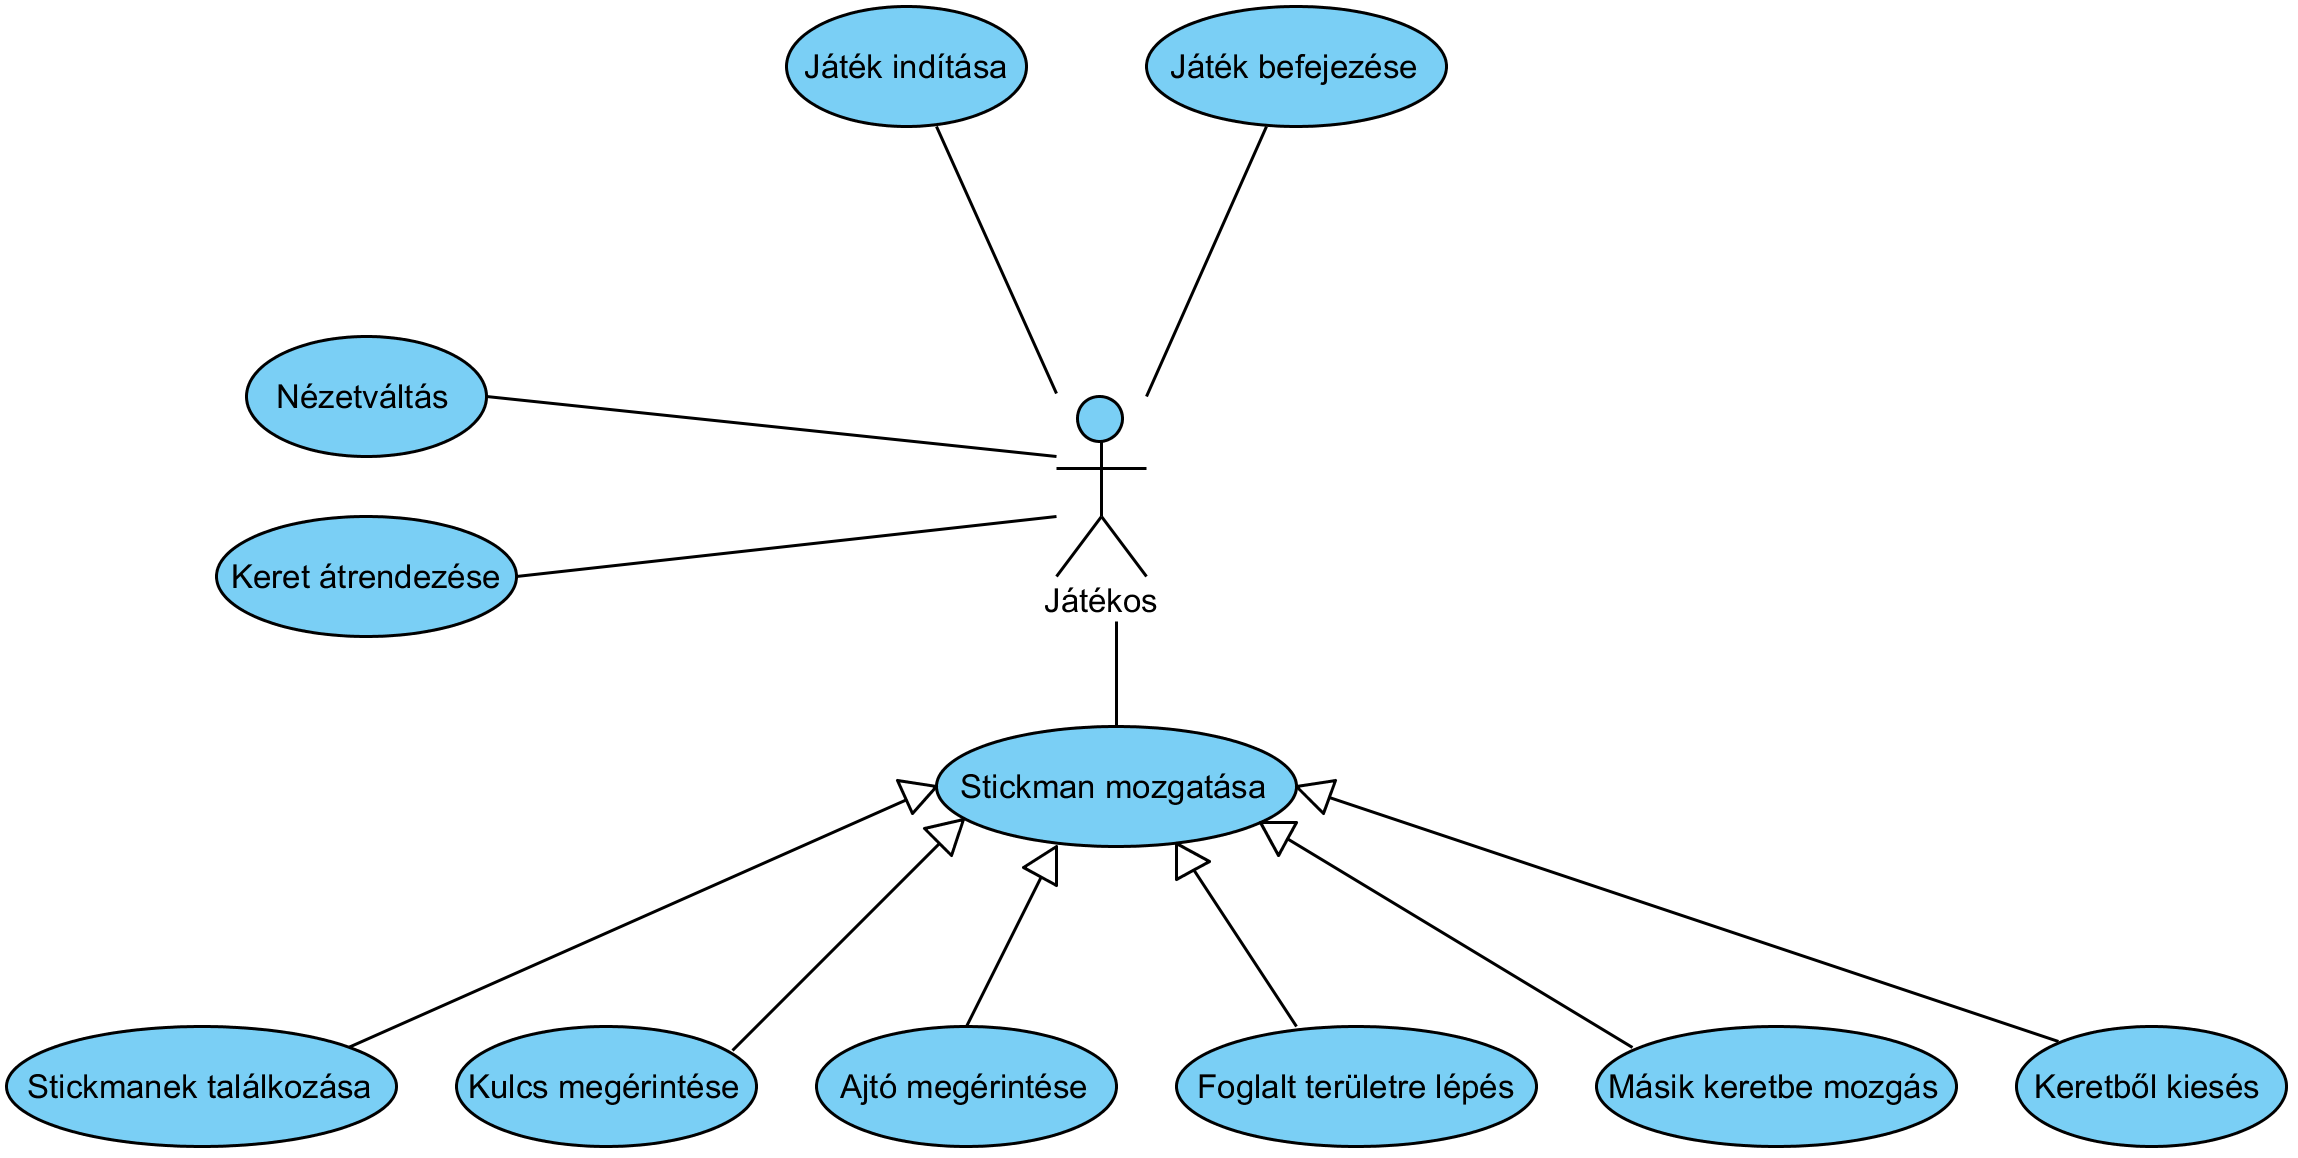
\includegraphics[scale=0.9]{resources/player.png}
		\end{center}        
        
        \subsubsection{Irányításhoz kapcsolódó use-case-ek} 
		
	    \begin{enumerate}[label=\textbf{\arabic*.}, start=1]
	        \ucitem{Játék indítása} 
	        \ucdesc{A felhasználó elindítja a játékot.} 
	        \ucact{Játékos}
	        \ucscenario{A pálya betöltődik, a stickmanek és a többi elem elhelyezésre kerül a pályán.} 

		
	        \ucitem{Játék befejezése} 
	        \ucdesc{Kilépés a játékból.} 
	        \ucact{Játékos}
	        \ucscenario{Az utolsó mentett pozíció alapján a játék mentése. Fájlok lezárása és kilépés a programból.} 
	        
	        \ucitem{Stickman mozgatása} 
	        \ucdesc{Játékos irányítja az egyik Stickmant.} 
	        \ucact{Játékos}
	        \ucscenario{A lehetséges irányok: jobbra, balra, fel(ugrás). Amennyiben a mozgás irányában van szabad terület, a pozíciója megváltozik, egyébként blokkolódik (helyben marad)}
		
	        \ucitem{Nézetváltás} 
	        \ucdesc{A játékos nézetet vált.} 
	        \ucact{Játékos}
	        \ucscenario{Ha közeli nézetben volt, akkor pálya nézetbe lép, ahol látja a kereteket. Ekkor a Stickman irányítása letiltódik és a keret átrendezés irányítása aktiválódik. Ha pálya nézetben volt, akkor fordítva.} 
	        
	        \ucitem{Keret átrendezése} 
	        \ucdesc{Pálya nézetben a keretek átrendezése.} 
	        \ucact{Játékos}
	        \ucscenario{A megadott irányok mentén a keretek átrendezhetőek, mindig az üres kerettel helyet cserélve} 
	    \end{enumerate}
	    
        \subsubsection{Időhöz kapcsolódó use-case-ek} 
		
	    \begin{enumerate}[label=\textbf{\arabic*.}, start=1]
	        \ucitem{Idő léptetése} 
	        \ucdesc{Jelzi az idő múlását.} 
	        \ucact{Óra}
	        \ucscenario{Számítógép által vezérelt idő léptetés, amely a Stickman vertikális pozícióját befolyásolja.} 
	    \end{enumerate}
	    
        \subsubsection{Stickman(ek)hez kapcsolódó use-case-ek} 

	    \begin{enumerate}[label=\textbf{\arabic*.}, start=1]
	    
	        \ucitem{Stickmanek találkozása} 
	        \ucdesc{Két Stickman mozgásuk során találkozik.} 
	        \ucact{Játékos}
	        \ucscenario{A két Stickman ütközik egymással, mint két szilárd objektum, de további interakció nem történik} 
		
	        \ucitem{Kulcs megérintése} 
	        \ucdesc{A Stickman mozgása során felvesz egy kulcsot.} 
	        \ucact{Játékos}
	        \ucscenario{A kulcs a stickmanhez kerül és eltűnik a pályáról}
		
	        \ucitem{Ajtó megérintése}
	        \ucdesc{A Stickman mozgása során egy ajtóhoz ér.}
	        \ucact{Játékos}
	        \ucscenario{Amennyiben minden kulcsot megszereztek, akkor vége a pályának, egyébként a Stickman elhalad az ajtó előtt.}

	        \ucitem{Keret elhagyása} 
	        \ucdesc{A Stickman valamely irányba elhagyja az aktuális keretet} 
	        \ucact{Játékos}
	        \ucscenario{Amennyiben van szomszédos keret és a két keret átjárható, a stickman belép az új keretbe. Amennyiben a szomszédos keret nem átjárható, akkor ha a célkeret alsószomszéd, a stickman kiesik, egyébként blokkolódik (helyben marad).}
	        
	    \end{enumerate}
	    
    	\subsection{Tesztelési terv}
			\newcommand{\testitem}[1]{\item \textbf{Név: #1}\\}
			\newcommand{\tdesc}[1]{\textbf{Leírás: } #1\\}
			\newcommand{\tcel}[1]{\textbf{Cél:} #1\\}
	
			\begin{enumerate}[label=\textbf{\arabic*.}, start=1]
%			    \testitem{}
%		        \tdesc{}
%		        \tcel{}
		        
		        \testitem{Pálya betöltése}
		        \tdesc{Betöltésre kerül egy objektumokkal feltöltött pálya, melyet a \texttt{MapFactory} készít el a pálya fájlreprezentációja alapján, és elhelyezi rajta a stickmaneket.}
		        \tcel{Ellenőrizni, hogy a pálya fájlreprezentációjából helyes pályakép generálódik a programban, minden objektum a helyén van-e. \texttt{MapFactory}-nak létre kell hoznia a megfelelő számú \texttt{Frame}-et és azokat helyesen elhelyezni, valamint létre kell hoznia a \texttt{FrameItem}eket.}
		        
		        \testitem{Stickman mozgatása kereten belül}
		        \tdesc{Az egyik stickmant megmozgatjuk kereten belül minden irányba: vízszintesen és horizontálisan (felfele), úgy hogy van tereptárgy a mozgás irányában, mely azt megakadályozza, és úgy is hogy nincs, illetve leugrunk vele egy magaslatról.}
		        \tcel{Ellenőrizni, hogy a kiadott mozgatási parancsok a várt helyre viszik-e a stickmant, a tereptárgyak megakadályozzák-e a mozgását, ill. hogy az ugrás helyesen működik-e (a parancs kiadása után az idő múlása során először fölfele mozog, majd megáll, lefele mozog, és talajt érve újra megáll). A teszt során a \texttt{Stickman} \texttt{area} attribútuma áll középpontban, illetve hogy a \texttt{PubSub}-ból jövő \texttt{tick} események hatására hogyan reagál.}
		        
		        \testitem{Stickman mozgatása keretek között}
		        \tdesc{A Stickmant először olyan keretek között mozgatjuk, melyek átjárhatóak, majd egy olyanba próbáljuk vezérelni, ahova nincs lehetősége átmenni.}
		        \tcel{Keretek közti átjárhatóság megállapítását végző algoritmus, ill. a \texttt{Stickman} egyik \texttt{Frame}-ből másikba való áthelyezésének ellenőrzése. \texttt{Frame} kérésére a \texttt{Map} visszaadja a szomszédos \texttt{Frame}-et, és az előbbi \texttt{Frame} átrakja oda a \texttt{Stickman}t.}
		        
		        \testitem{Stickman kiesése}
		        \tdesc{Stickmant úgy vezéreljük, hogy essen ki egy keret alján úgy, hogy arra nincs több keret, vagy afelé a keret nem átjárható.}
		        \tcel{Ellenőrizzük, hogy a {Stickman} kiesik-e, ha a játék szabályai szerint ki kell esnie, illetve megnézzük, hogy ilyenkor visszakerül-e az utolsó ellenőrzőponthoz. Az aktuális \texttt{Frame} elkéri a \texttt{Map}től a szomszédját, melyre az \texttt{null} értékkel válaszol, erről pedig értesíti a \texttt{Stickmant}.}
		        
		        \testitem{Kulcs felvétele, pálya teljesítése}
		        \tdesc{Stickmannel először megérintjük az ajtót, ezután felvesszük a kucsot, majd megint megérintjük az ajtót.}
		        \tcel{Ellenőrizzük, hogy az ajtó csak kulccsal nyitható-e, illetve hogy a kulcs felvétele megfelelően rögzítődik-e. A teszt középpontjában a \texttt{Frame} által megvalósított ütközésértesítés áll, illetve az állapotok rögzítése, mely a \texttt{PubSub}-on jövő értesítés után a \texttt{Game}-ben történik.}
		        
		        \testitem{Keret mozgatása}
		        \tdesc{Távoli nézetben keret mozgatása parancsot adunk ki.}
		        \tcel{Ellenőrizzük, hogy a keret mozgatása parancs hatására a \texttt{Map} a megfelelő \texttt{Frame}-et mozgatja és azt a megfelelő helyre viszi.}
		        
		        \testitem{Nézetek közötti váltás}
		        \tdesc{A pálya betöltése után a kezdeti távoli nézetből közelibe váltunk. Itt ugrunk egyet, majd megpróbáljuk a kereteket átrendezni, ami nem sikerül. Esünk egyet, mely közben távoli nézetbe váltunk. Ekkor megpróbáljuk vízszintesen mozgatni a stickmant, ami nem sikerül.}
		        \tcel{Ellenőrizzük, hogy a stickman mozgatása le van-e tiltva távoli nézetben, illetve a keretek mozgatása közeli nézetben. Megnézzük még, hogy az időzítés helyesen működik-e, a kiadott \texttt{tick} parancs ellenére sem esik tovább a \texttt{Stickman} távoli nézetben.}
			\end{enumerate}
	    	
	\subsection{Tesztelést támogató segéd- és fordítóprogramok specifikálása}		
A tesztelés során keletkező kimenetek összehasonlítása az előre definiált kimenetekkel nem kézi erővel történik, erre a unix(-like) rendszereken megtalálható \texttt{diff} -- vagy azzal azonos funkcionalitású, más platformon futó -- programot fogunk használni. Egy teszteset akkor tekinthető sikeresnek, ha a \texttt{diff} program nem jelez különbséget a kapott kimenet és az előre definiált kimenet között.

	\subsection{Napló}
	% The diary generator uses the following comments to identify the beginning and the ending of the generated diary
	% The following content is auto generated, please do NOT modify, edit the related shared document instead.
	%GENERATOR:DIARY
    \begin{center} 
        \begin{tabular}{| l | p{1.9cm} | p{2.6cm} | p{6.1cm} |}
            \hline
                Kezdet & Időtartam & Résztvevők & Leírás \\
            \hline \hline 
2012. 03. 20. 17:00 & 4 óra & Thaler & Prototípus tervezés\\ \hline
2012. 03. 21. 14:00 & 3 óra & Thaler & Prototípus kialakítás\\ \hline
2012. 03. 24. 08:00 & 0.5 óra & Thaler & Inicializálás\\ \hline
2012. 03. 24. 19:45 & 3 óra & Thaler & Interface def\\ \hline
2012. 03. 24. 22:00 & 1.5 óra & Fodor, Kádár, Thaler & Team meeting\\ \hline
2012. 03. 25. 11:00 & 0.5 óra & Fodor & Tesztelési terv\\ \hline
2012. 03. 25. 12:00 & 2 óra & Kádár & Use case-ek\\ \hline
2012. 03. 25. 14:00 & 4 óra & Thaler & Prototípus felület\\ \hline
2012. 03. 25. 15:00 & 3 óra & Fodor & Tesztelési terv\\ \hline
2012. 03. 25. 20:30 & 1 óra & Thaler & Takarítás, csomagolás\\ \hline
2012. 03. 25. 21:00 & 0.5 óra & Fodor & Dokumentum átnézése\\ \hline
2012. 03. 25. 21:30 & 0.5 óra & Kádár & Use case javítás\\ \hline
2012. 03. 26. 00:00 & 1 óra & Berki & Nyomtatás, minőségellenőrzés\\ \hline

            \hline
        \end{tabular}
    \end{center}
%GENERATOR:DIARY
\end{document}
